\section{Intro}
\subsection{Begriffe}
\begin{concept}{Grundlegende Begriffe}\\
\begin{tikzpicture}
  % Itemized list
  \node[anchor=north west] (list) at (0, 0) {
    \begin{minipage}{\textwidth}
      \begin{itemize}
        \item $\Omega =$ Grundgesamtheit
        \item $n =$ Anzahl Objekte
        \item $X =$ Stichprobenwerte
        \item $a =$ Ausprägungen
        \item $h =$ Absolute Häufigkeit
        \item $f =$ Relative Häufigkeit
        \item $H =$ Kumulative Absolute Häufigkeit
        \item $F =$ Kumulative Relative Häufigkeit
      \end{itemize}
    \end{minipage}
  };

  % Image
  \node[anchor=north west] (image) at (4, 0) {
    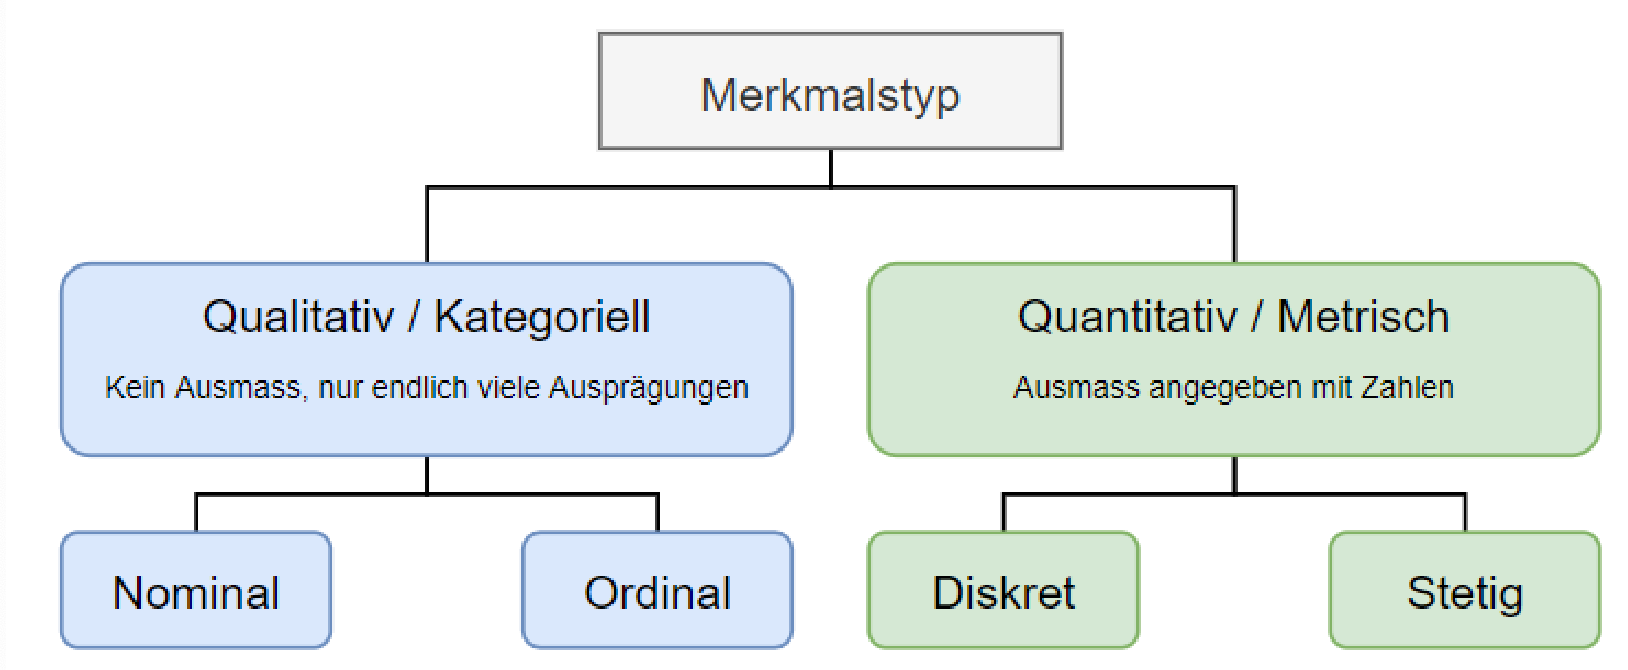
\includegraphics[width=0.5\textwidth]{images/merkmalstypen.png}
  };
\end{tikzpicture}
\end{concept}

\begin{definition}{Boxplot}\\
\begin{minipage}{0.6\columnwidth}
\begin{itemize}
  \setlength{\itemsep}{5pt}
  \item $\textcolor[HTML]{A70000}{Q_{1}},\textcolor[HTML]{005700}{ Q_{2}=x_{\text {med }}},\textcolor[HTML]{A70000}{ Q_{3}}$
  \item $I Q R=Q_{3}-Q_{1}$
  \item Untere Antenne $\textcolor[HTML]{0707FF}{x_{u}}:\\ u=\min \left[Q_{1}-1.5 \cdot I Q R, Q_{1}\right]$
  \item Obere Antenne $\textcolor[HTML]{0707FF}{x_{0}}:\\ \quad o=\max \left[Q_{3}+1.5 \cdot I Q R, Q_{3}\right]$
  \item Ausreisser: $\quad x_{i}<\textcolor[HTML]{0707FF}{x_{u}} \vee x_{i}>\textcolor[HTML]{0707FF}{x_{0}}$
\end{itemize}
\end{minipage}%
\begin{minipage}{0.4\columnwidth}
  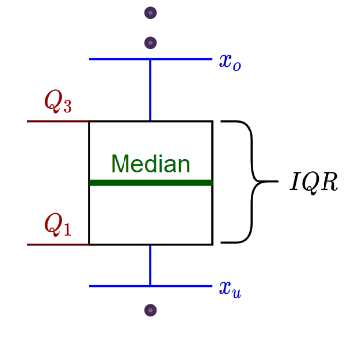
\includegraphics[width=\textwidth]{images/boxplot.png}
\end{minipage}
\end{definition}

%%basic formulas and shit
